\chapter{各向同性线性硬化材料杆的有限元分析}
\label{cha:abaqus_hardened}
其他条件不变,将材料考虑为各向同性线性硬化材料,硬化模量取为~{$K=0.05E$},再进行有限元分析。圆杆~S33~应力云图、S23~应力云图和圆杆跨中截面正应力与剪应力分布云图如图~\ref{fig:k}~所示。
\begin{figure}[htbp]
    \centering
	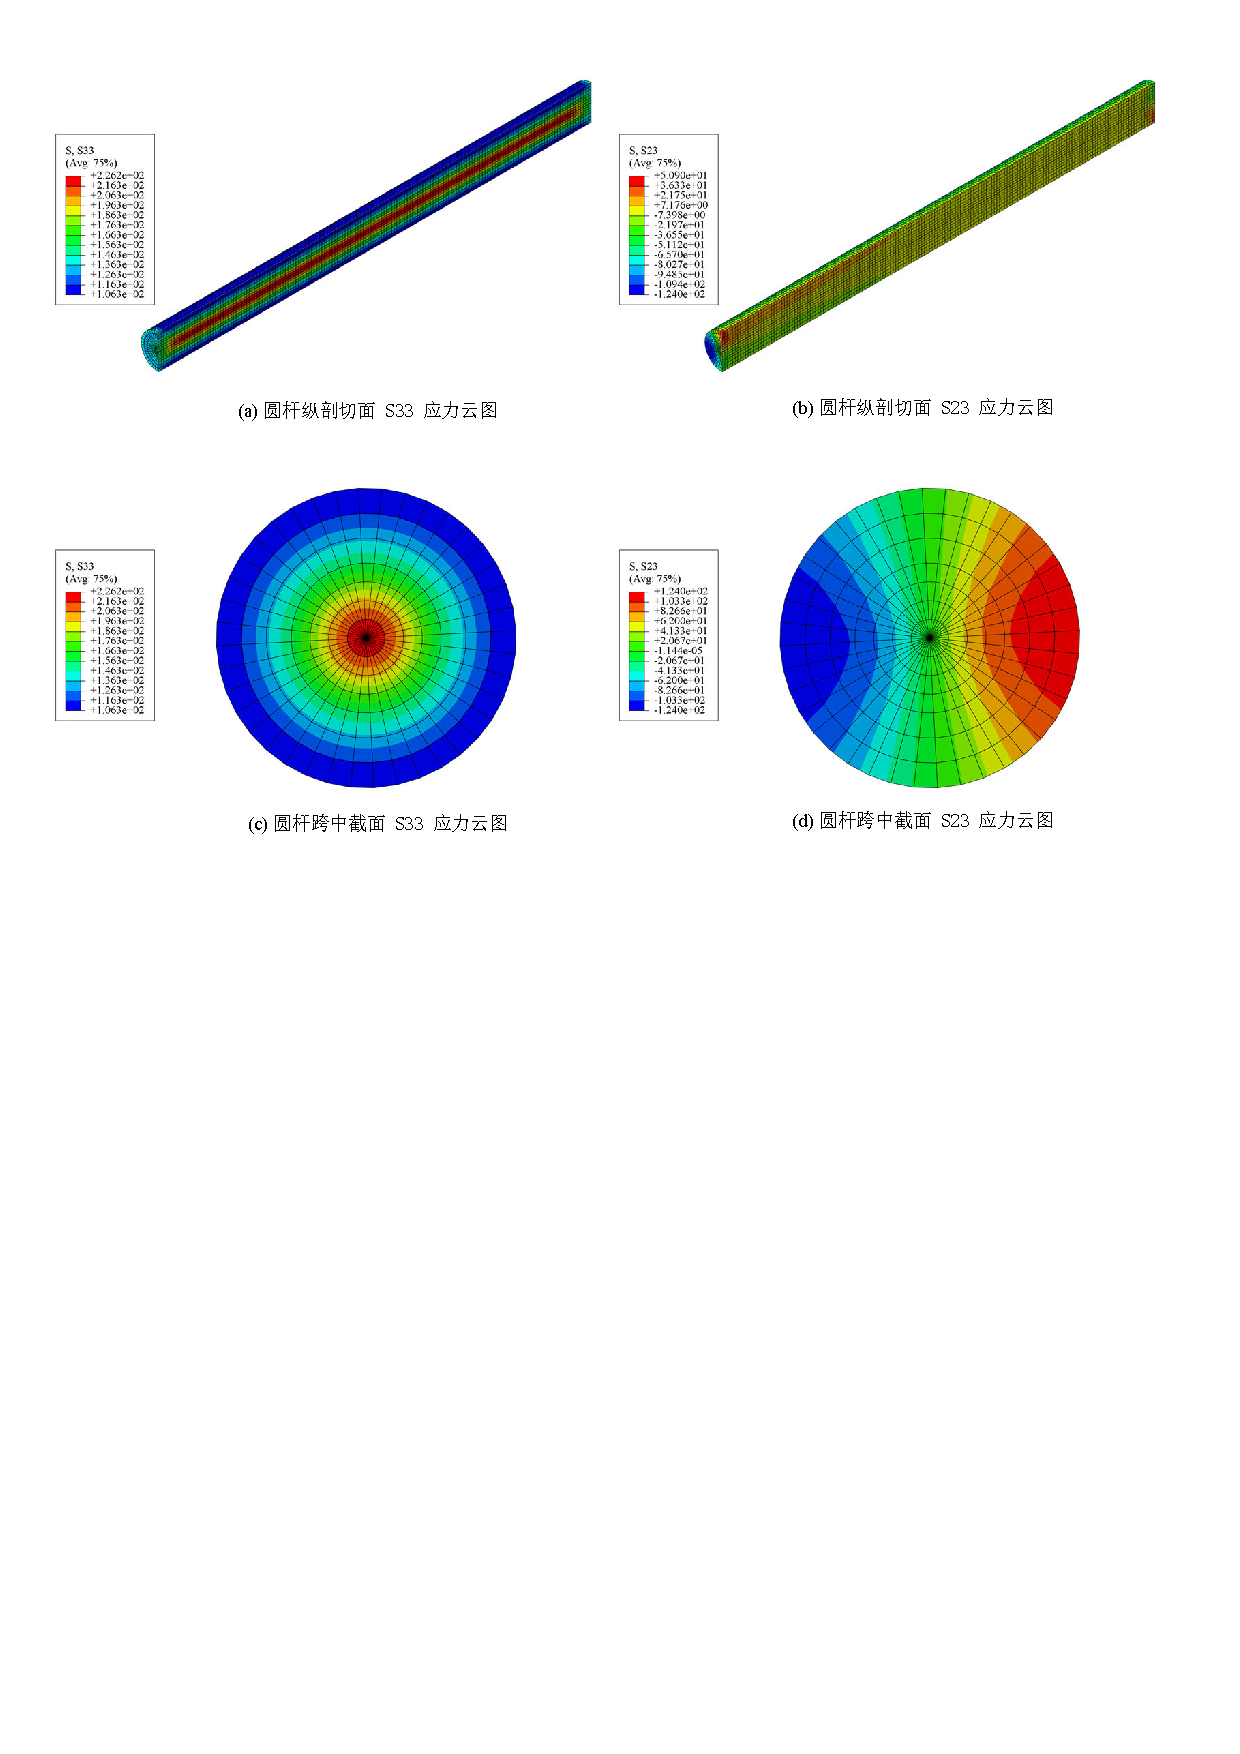
\includegraphics[width=1\textwidth]{k.pdf}
    \caption{考虑线性硬化圆杆数值模拟应力结果}
    \label{fig:k}
\end{figure}

导出各向同性线性硬化材料条件下,圆杆跨中截面正应力与剪应力的径向分布结果,并与理想弹塑性材料条件下的有限元分析结果进行比较,绘制散点图如图~\ref{fig:ks3323}~所示。

观察曲线图可以发现,在考虑材料各向同性线性硬化之后,截面正应力和剪应力的分布仍然符合根据理想弹塑性材料计算得到的规律。整体而言,考虑硬化之后的截面正应力与剪应力大于仅考虑理想弹塑性的应力计算结果。并且二者差距随着距离圆心距离的增大而增大,这是由于越靠近截面边缘,塑性应变越大,材料强度硬化越显著。

进一步总结可得,理想弹塑性材料的假设适用于初步的工程分析和简单的结构计算,但通常不考虑材料的塑性硬化特性,适用于对材料性质要求较为宽松的场合\cite{Mohr2008,Hill1950}。对于该问题的分析,弹塑性硬化材料模型通常更为合理,因为它能更真实地模拟材料在屈服后的表现,并能更好地反映出扭转过程中材料的变形和强度变化。
\begin{figure}[htbp]
    \centering
	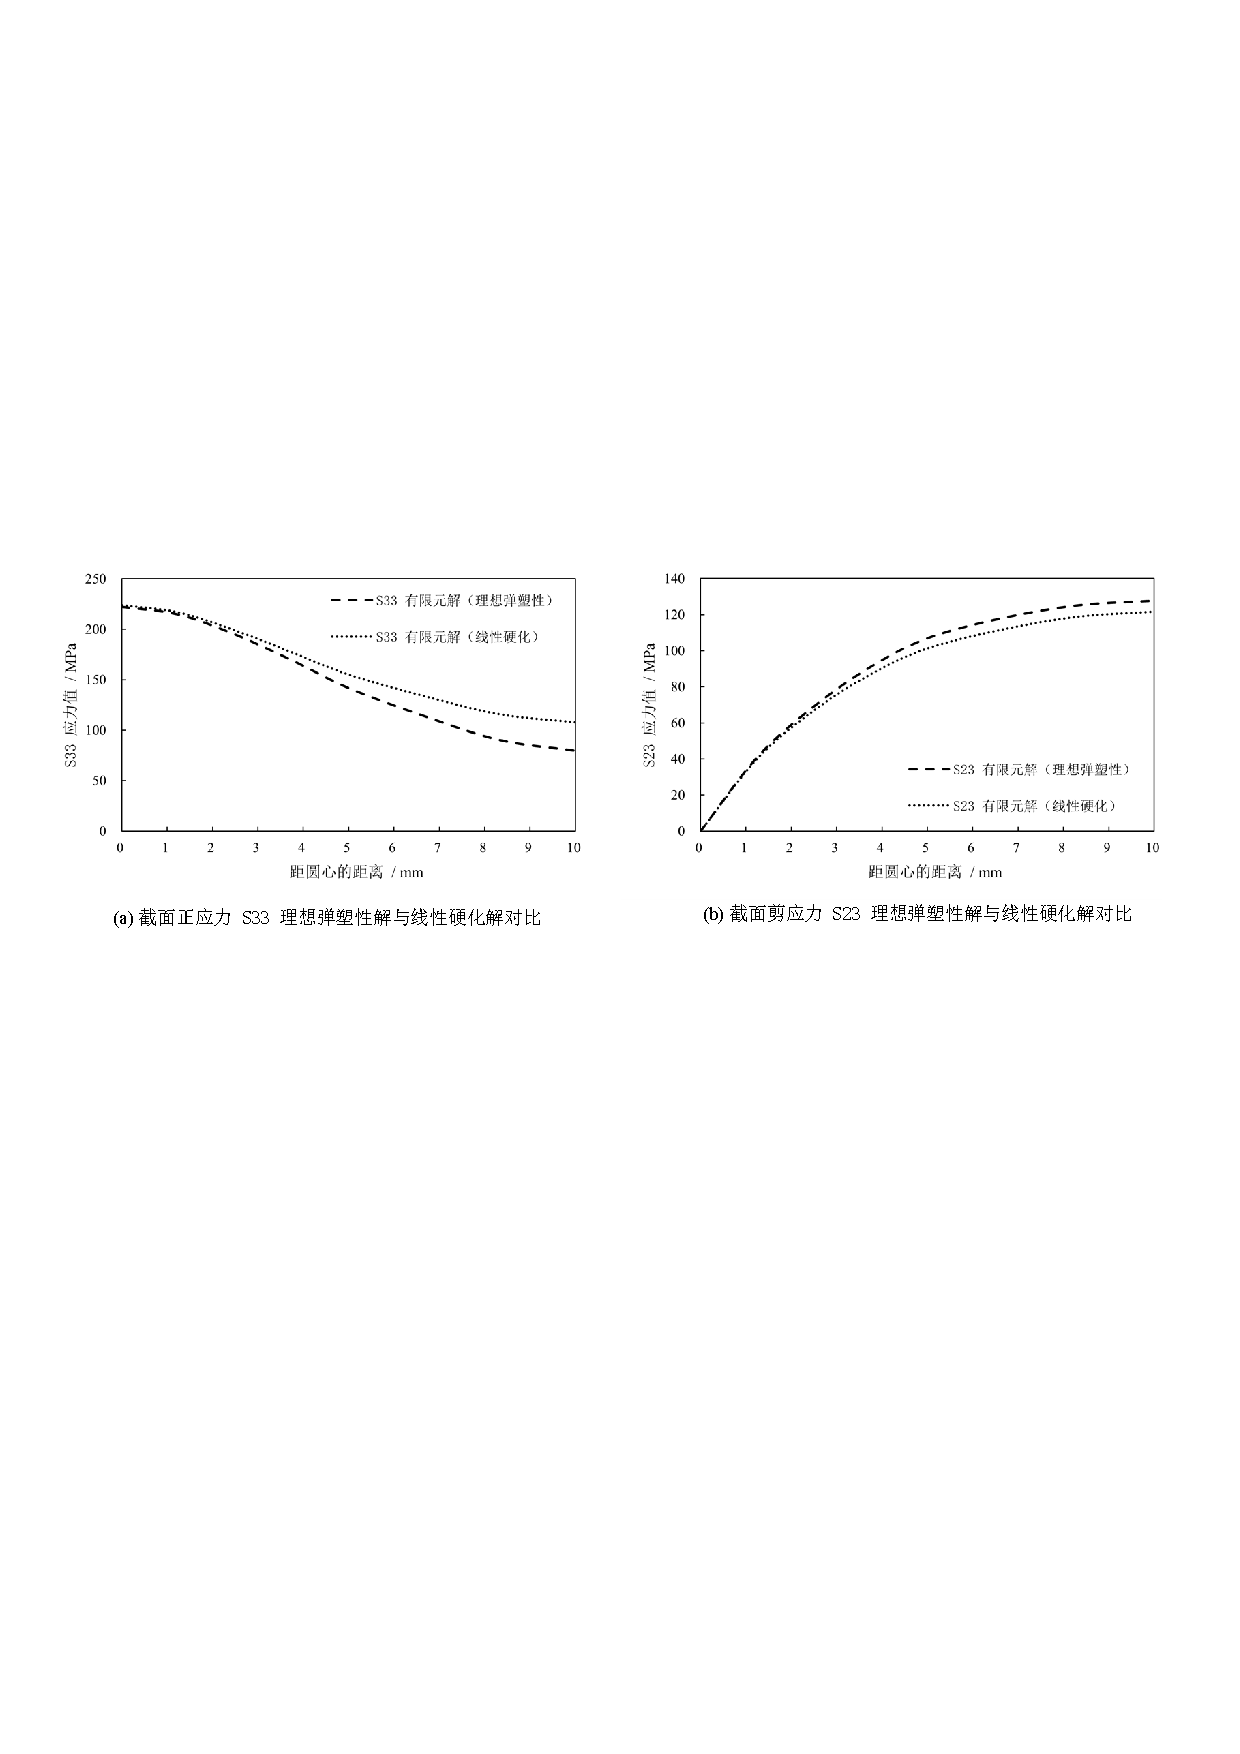
\includegraphics[width=1\textwidth]{2.pdf}
    \caption{理想弹塑性解与线性硬化解对比}
    \label{fig:ks3323}
\end{figure}